
%
% state - vis
%

\section{Visual mapping}

N\"{o}llenburg~\cite{noellenburg11geovis} names three ``Driving forces in geovisualization'': The advent of high speed parallel processing and technology advances in computer graphics, today allows us to grasp enormous amounts of information. Besides the advances in graphics and display technologies, the second main driving force in geographic visualization is the increasing amount of geospatial data being collected and available. Finally, the third force is the \textit{rise of the Internet}, which significantly pushes web mapping and contributes to geovisualization technologies.

As a logical consequence of broader audiences having access to geospatial visualizations using the Internet, it appears that there is a shift from technology-driven visualization towards more human-centered approaches. Interactive and highly dynamic interfaces have helped the map evolve from its traditional role as a presentational device towards exploring geospatial data~\cite{noellenburg11geovis, vislecture}.

In chapter \ref{chapter:foundations-vis}, foundations of visualization, visual variables and data exploration techniques as well as the concept of clutter reduction have been introduces. In the following, existing visualization techniques for representing clustered data on maps will be discussed. In a first step, visualization concepts on the map level will be discussed. Later, approaches for visualizing individual clusters will are added. 

\subsection{Map visualization types for clustering}
\label{chapter:map-vis}

There exists a variety of map types, serving different purposes like standard geographic maps, cartograms, geologic maps, linguistic maps or weather maps. Some of these use distortion, for example the cartogram can be used to map the area of each country to the size of population. In this section, we try to identify those map types which are appropriate for visualizing clustered data\cite{noellenburg11geovis, wiki:map-types}:

\begin{itemize}

\item \textbf{Geographic map with markers}. The default way of representing data is a standard 2-dimensional map with markers on top of it. Each marker represents a data point or in the case of clustering, a cluster.

\parbox [h]{0.4\textwidth}{
    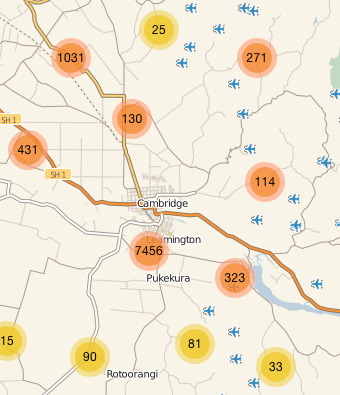
\includegraphics [width=\linewidth]{figures/map_types_normal_leaflet.png}
    \captionof {figure}{Leaflet map}
    \label{fig:map-type-standard-leaflet}
}
\hfill
\hspace{0.5cm}
\parbox [h]{0.4\textwidth }{
    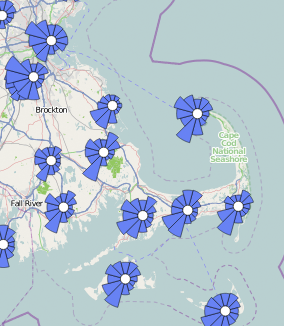
\includegraphics [width=\linewidth]{figures/map_types_standard_wind.png}
    \captionof {figure}{Wind history map}
    \label{fig:map-type-standard-wind}
}

\begin{itemize}

\item Figure \ref{fig:map-type-standard-leaflet} depicts an example\footnote{Leaflet.clustermarker example map from \url{http://leaflet.github.io/Leaflet.markercluster/example/marker-clustering-realworld.10000.html}} of the Leaflet.markercluster library. Clustered results are displayed using markers of the same size. The amount of items within a cluster is indicated by using a ``hot-to-cold'' color ramp~\cite{web:color-ramp}. 

\item Figure \ref{fig:map-type-standard-wind} shows a similar example, in this case a Wind history map\footnote{Wind history map \url{http://windhistory.com/map.html}} with markers for every wind measurement point. In this case, an advanced visualization technique is used for visualizing the amount of wind per cardinal direction as polar area diagrams.

\end {itemize}

The comparison between the two standard maps shows the potential of using advanced visualization techniques for displaying cluster items. Further ways for cluster visualization will be discussed in chapter \ref{chapter:cluster-vis}.

\item \textbf{Geographic Heatmap}

Heatmaps use colored, two-dimensional areas to express the value of each data entity on the map. Choropleth maps are the most common heatmaps, which are often used for analysis of geographic and statistical data. 

\parbox [h]{0.4\textwidth}{
    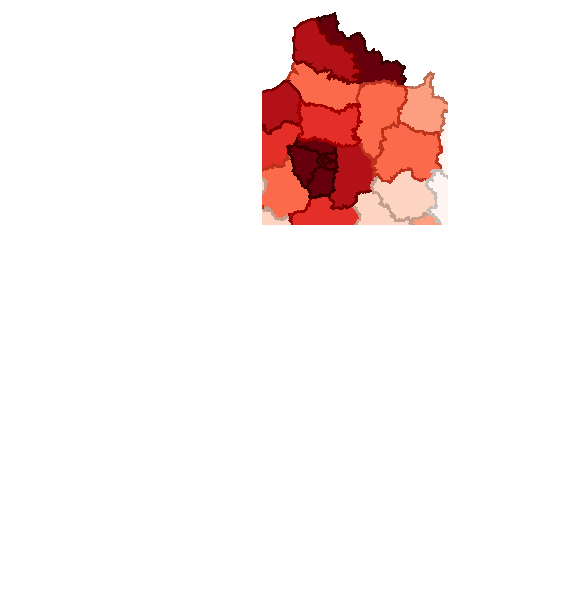
\includegraphics [width=\linewidth]{figures/map_types_choropleth.pdf}
    \captionof {figure}{Choropleth map}
    \label{fig:map-type-choropleth}
}
\hfill
\hspace{0.5cm}
\parbox [h]{0.4\textwidth}{
    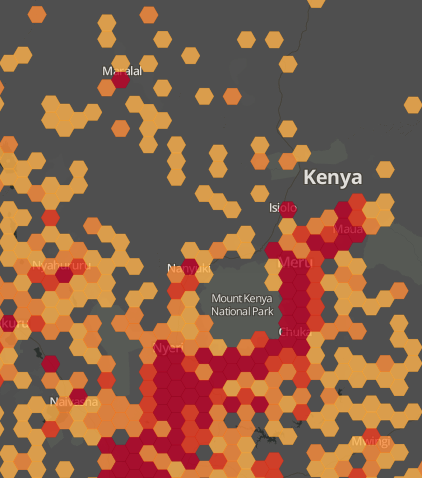
\includegraphics [width=\linewidth]{figures/map_types_heatmap.png}
    \captionof {figure}{Heatmap}
    \label{fig:map-type-binning}
}


\begin{itemize}

\item Figure \ref{fig:map-type-choropleth} visualizes an example choropleth map\footnote{Choropleth map example from Kartograph \url{http://kartograph.org/showcase/choropleth/}} that shows population data for each of the departments of metropolean France. Color coding is used to indicate densely populated regions with heavier red tones.

\item Figure \ref{fig:map-type-binning} presents another example\footnote{Heatmap that uses binning \url{http://mapbox.com/blog/binning-alternative-point-maps/}} that uses \textit{binning} for creating a hexagonal tessellation of the surface in order to visualize clustered results. 

\end {itemize}

A problem with heat maps is that they require a non-overlapping tessellation of the surface to provide the areas for visualization. As the binning example indicates, such a tessellation can also be done programmatically. Heatmap therefore can also be used for visualizating arbitrary clustered data without a need to calculate the exact boundaries of clusters. Another variation of heatmaps is the prism map, which adds extrusion of areas as a third-dimension~\cite{ladenhauf12dia, Delort10vis}. A publication on the evaluation of color schemes in choropleth maps can be found in~\cite{MacEachrenMort}. 


\item \textbf{Dot Grid maps}

Dot Grid maps are based on the suggestion by Jaques Bertin~\cite{bertin67graphics, bertin83graphics} to use graduated sizes in a regular pattern as an alternative to chloropeth maps. The advantage is, that the map creator doesn't have to choose between quantity or density of a distribution value, because the dot grid map shows both a the same time. The user can understand the data distribution on a finer level of granularity, as opposed to where the chloropeth map usually creates larger areas of aggregated information~\cite{web:dot-grid}.

Figure \ref{fig:map-type-dotgrid} is an alternative version\footnote{Dot Grid map example from Kartograph \url{http://kartograph.org/showcase/dotgrid/}} of the France map from figure \ref{fig:map-type-choropleth}, visualized as a dot grid map.


\item \textbf{Voronoi map}

The Voronoi tessellation is a space partitioning technique. From a set of points, it produces a Voronoi polygon for each point, such that the area covered is closest to that point in comparison to all other points. Jean-Yves Delort describes a technique that uses Voronoi polygons for ``Vizualizing Large Spatial Datasets in Interactive Maps''~\cite{Delort10vis}. It uses a hierarchical clustering technique to choose a subset of points per zoom level for proper visualization. Still, the effectiveness of this approach is questionable, as the scalability analysis of the studies shows that the technique can efficiently be used for datasets of up to 1000 items.

Figure \ref{fig:map-type-voronoi} show an exemplary voronoi map\footnote{Voronoi map example \url{http://mbostock.github.io/d3/talk/20111116/airports-all.html}} that displays all U.S. airports as of 2008. Besides the shown visualization, for Voronoi maps apply the same visualization possibilities as for cloropeth maps.

\parbox [h]{0.4\textwidth }{
    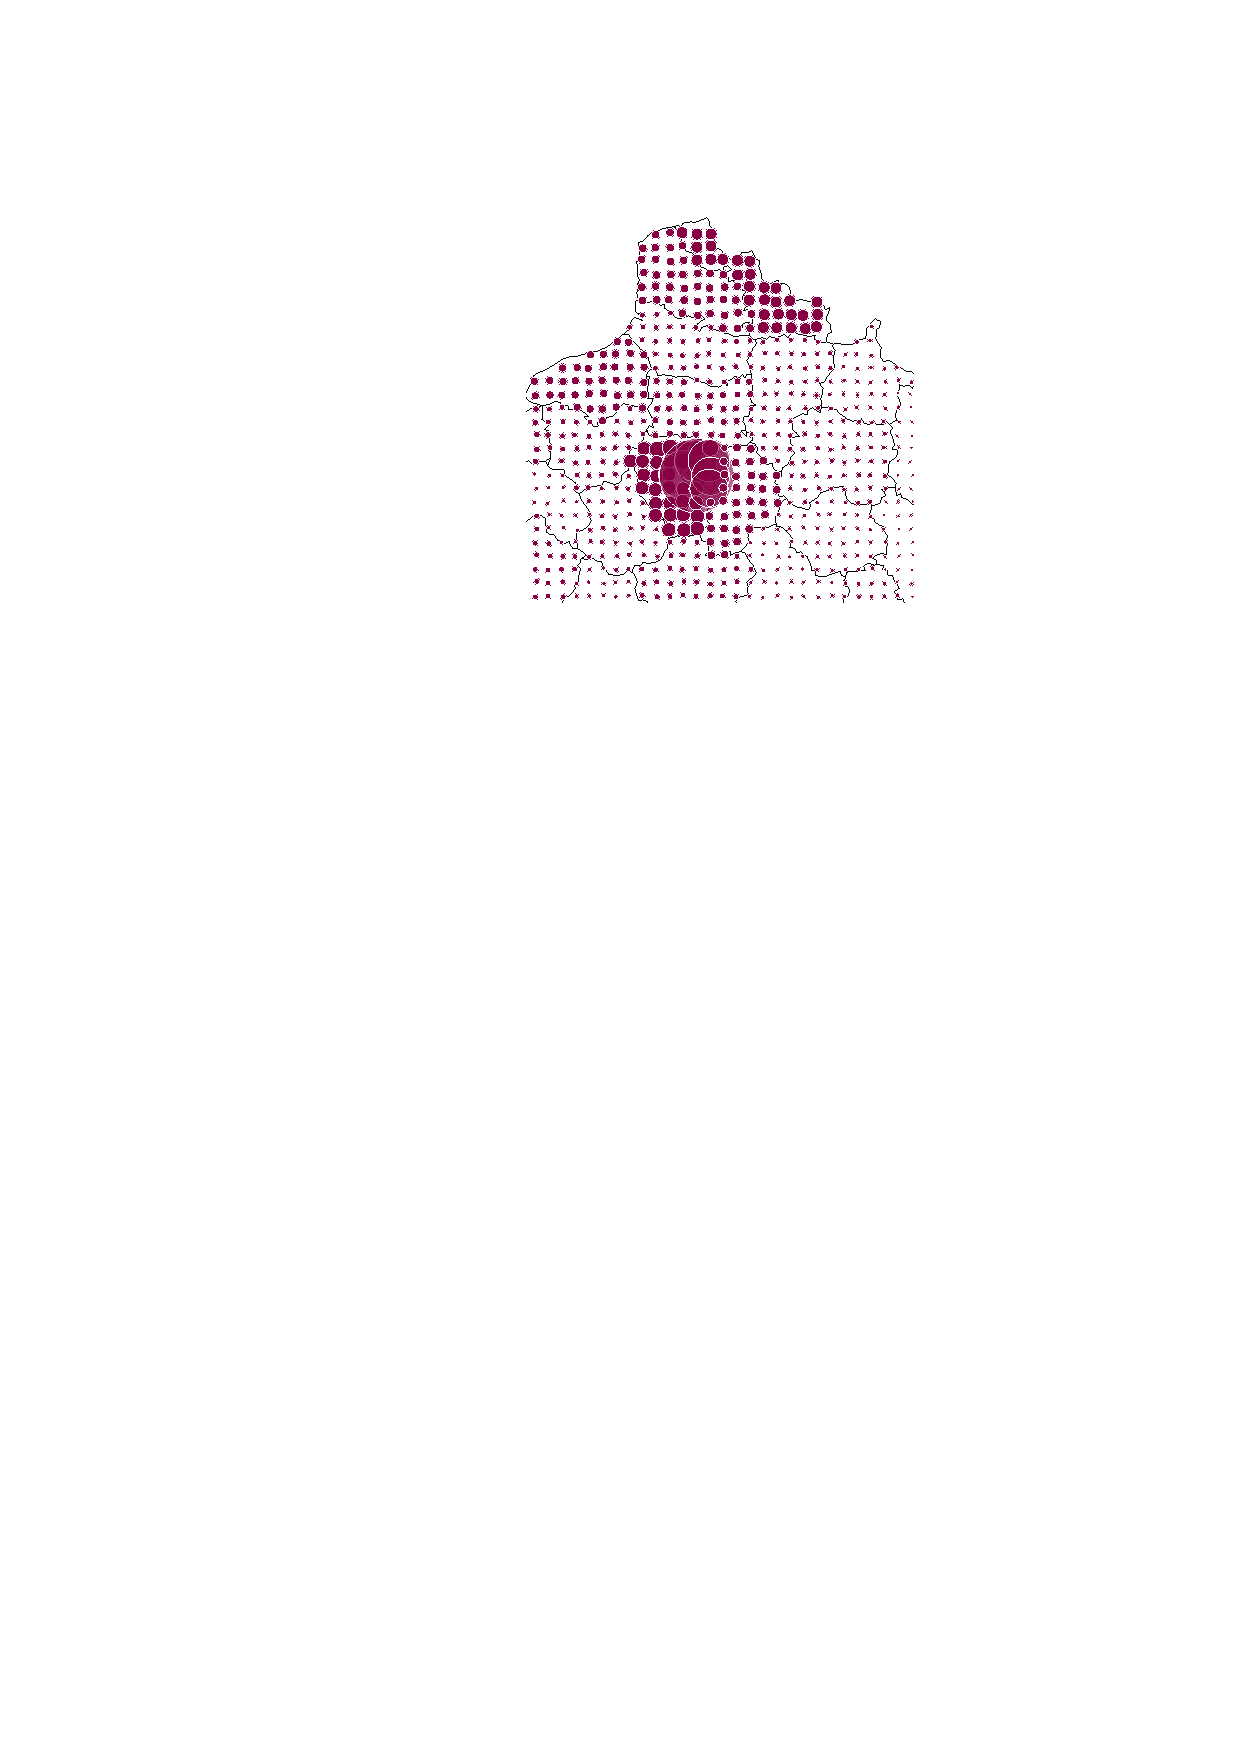
\includegraphics [width=\linewidth]{figures/map_types_dot_grid.pdf}
    \captionof {figure}{Dot Grid map}
    \label{fig:map-type-dotgrid}
}
\hfill
\hspace{0.5cm}
\parbox [h]{0.4\textwidth }{
    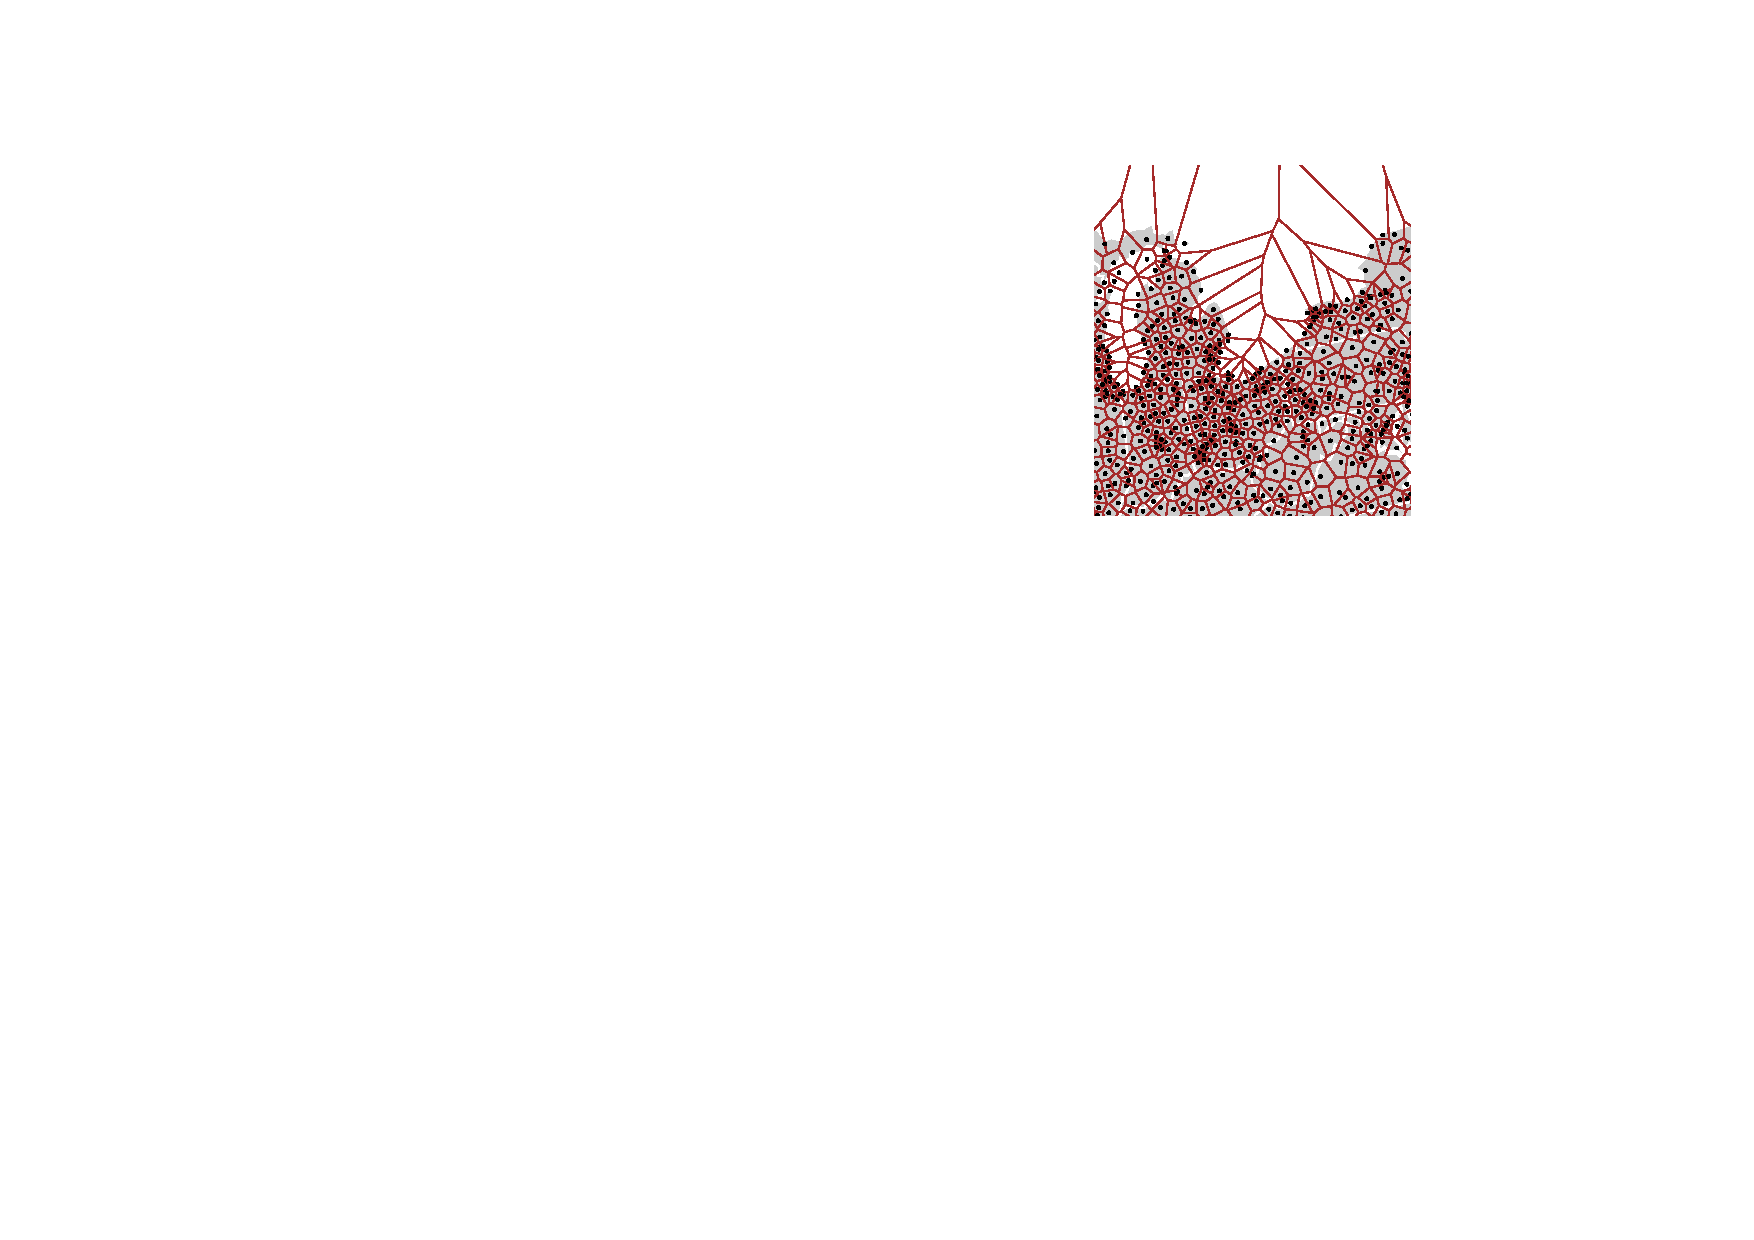
\includegraphics [width=\linewidth]{figures/map_types_voronoi.pdf}
    \captionof {figure}{Voronoi map}
    \label{fig:map-type-voronoi}
}

\end{itemize}

Self-organizing maps (SOM) can also be used to visualize clusters of data. But instead of displaying data on a geographic map, self-organizing maps create their own virtual space in order to represent information~\cite{noellenburg11geovis}.  


\subsection{Cluster visualization techniques for maps}
\label{chapter:cluster-vis}

The previous chapter has shown different kinds of map visualization techniques appropriate for displaying clustered data. In the end, each visualization will show (clustered) items on a map as objects with attributes like a particular shape or coloring. As clusters contain aggregated information, the task is to find the right way for visualizing the cluster items themselves. From the examples so far, we have seen variations in size, shape and color which expose information on the cluster items being visualized on the map. In the following, multivariate data visualization techniques will be evaluated for visualizing cluster items on a map.

In chapter \ref{vis-data-techniques}, a classification of visualization techniques by data type and interaction technique has been presented. Ke-Bing Zhang~\cite{zhang07thesis} has written about ``Visual Cluster Analysis in Data Mining'' where he list an extensive list of multivariate data visualization techniques. Potentially any such visualization technique can be used, but the frame of the map puts constraints in terms of space on the representation of individual items. Iconic displays are a simple way to visualize data, which also prevents clutter. Dense Pixel displays and geometric visualizations like charts can be used to encode more complex information.

\begin{itemize}

\item \textbf{Icon-based, Glyphs}

Matthew O Ward\cite{ward02glyphs} defines \textit{glyphs} as ``graphical entities that convey one or more data values via attributes such as shape, size, color, and position''. While the work of Otto Neurath on ISOTYPE~\cite{neurath} (1930s) can be seen as fundamental for pictorial statistics, the best-known literature reference to glyphs is ``Chernoff faces''\cite{chernoff73}. As indicated in (e) of figure \ref{fig:glyphs-ward}, data is encoded into properties of the face icon, such as shape of nose, mouth, eyes. Other fundamental glyph-based techniques include stick figures~\cite{stickfigures}, color icons~\cite{coloricons}, Hyperbox~\cite{hyperbox} and shape coding~\cite{shapecoding}. Figure \ref{fig:glyphs-ward} extends this list by showing examples of glyphs that Ward collected for his taxonomy of glyphs placement strategies\cite{ward02glyphs}.

\begin{figure}[h]
  \begin{center}
    \hspace*{-1cm}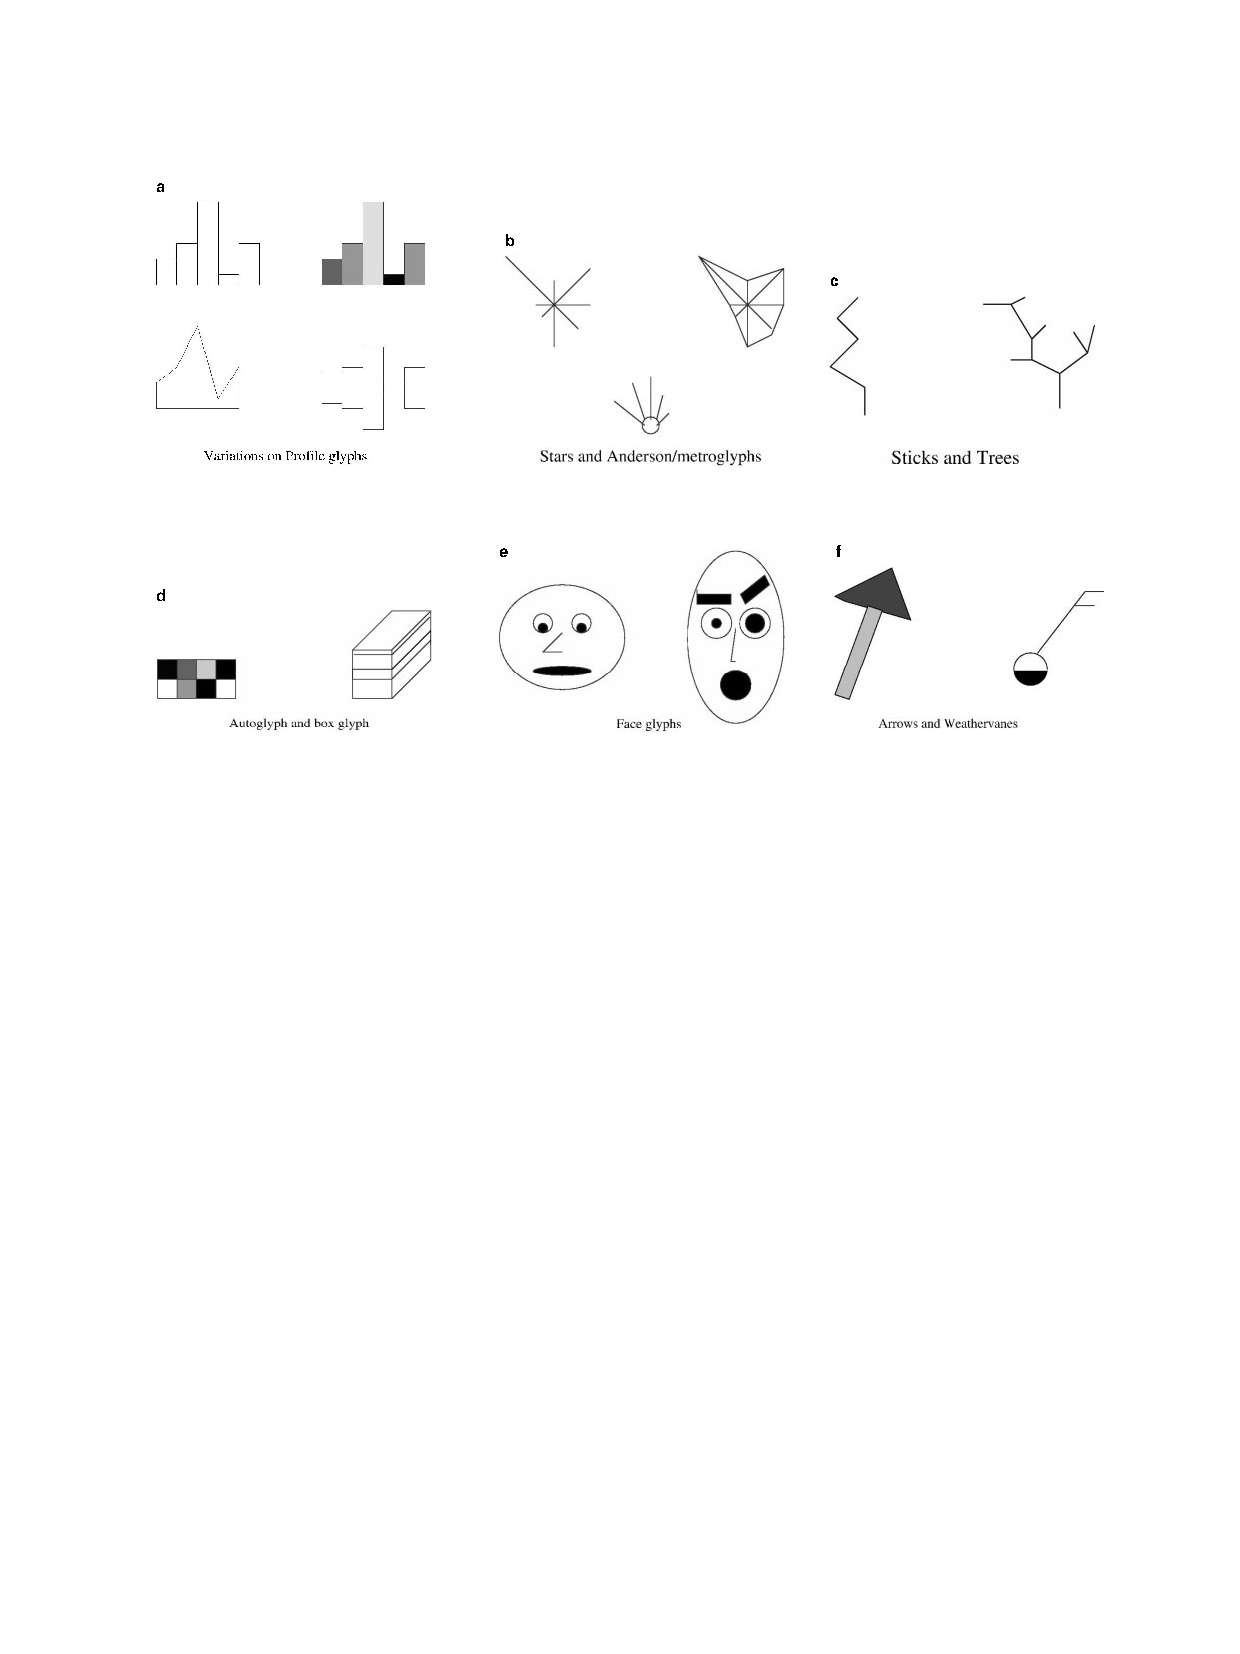
\includegraphics[width=1.2\textwidth]{figures/glyphs.pdf}
    \caption{Examples of glyphs. Top row: (a) variations on profiles; (b) stars/metroglyphs; and (c) stick figures and trees.
Bottom row: (d) autoglyphs and boxes; (e) faces; and (f) arrows and weathervanes.~\cite{ward02glyphs}.}
    \label{fig:glyphs-ward}
  \end{center}
\end{figure}

Some glyph types have been created to identify clusters or similarities by plotting them side-by-side on a 2-dimensional plane, a technique which is referred to as mosaic-based rendering. Stick figures and mosaic metaphors are examples in that field~\cite{stickfigures, nocke05mosaic}. One the other hand, reducing visual clutter as explained in chapter \ref{clutter-reduction} also matters for glyphs, especially when putting them on a map. A trade-off between information-richness vs. simplicity and clarity has to be made. As Zhang writes ``the amount of data increasing, the user hardly makes any sense of most properties of data intuitively, this is because the user cannot focus on the details of each icon when the data scale is very large''~\cite{zhang07thesis}. We can compare this to the map use cube presented in chapter \ref{chapter:foundations-vis}: more complex glyph types seem to be better suited for scientific purposes which can be related to private uses, while simpler glyph types can be used for presenting data to a public audience.

Examples for uses of simple icons and glyph types for clustered data on maps can be found in JavaScript mapping libraries as seen in chapter \ref{chapter:client-side-web-mapping}. These are usually based on a simple icon or geometric shape like a circle or marker and use color coding and size variations as indicators for underlying information. Figure \ref{fig:glyphs-zame} visualizes eight simple glyphs~\cite{ElmqvistDGHF08}. Further examples are scaled data values and scaled dots \cite{web:scaled-data-value}, as well as the proportional symbol map \cite{vislecture}.

\begin{figure}[h]
  \begin{center}
    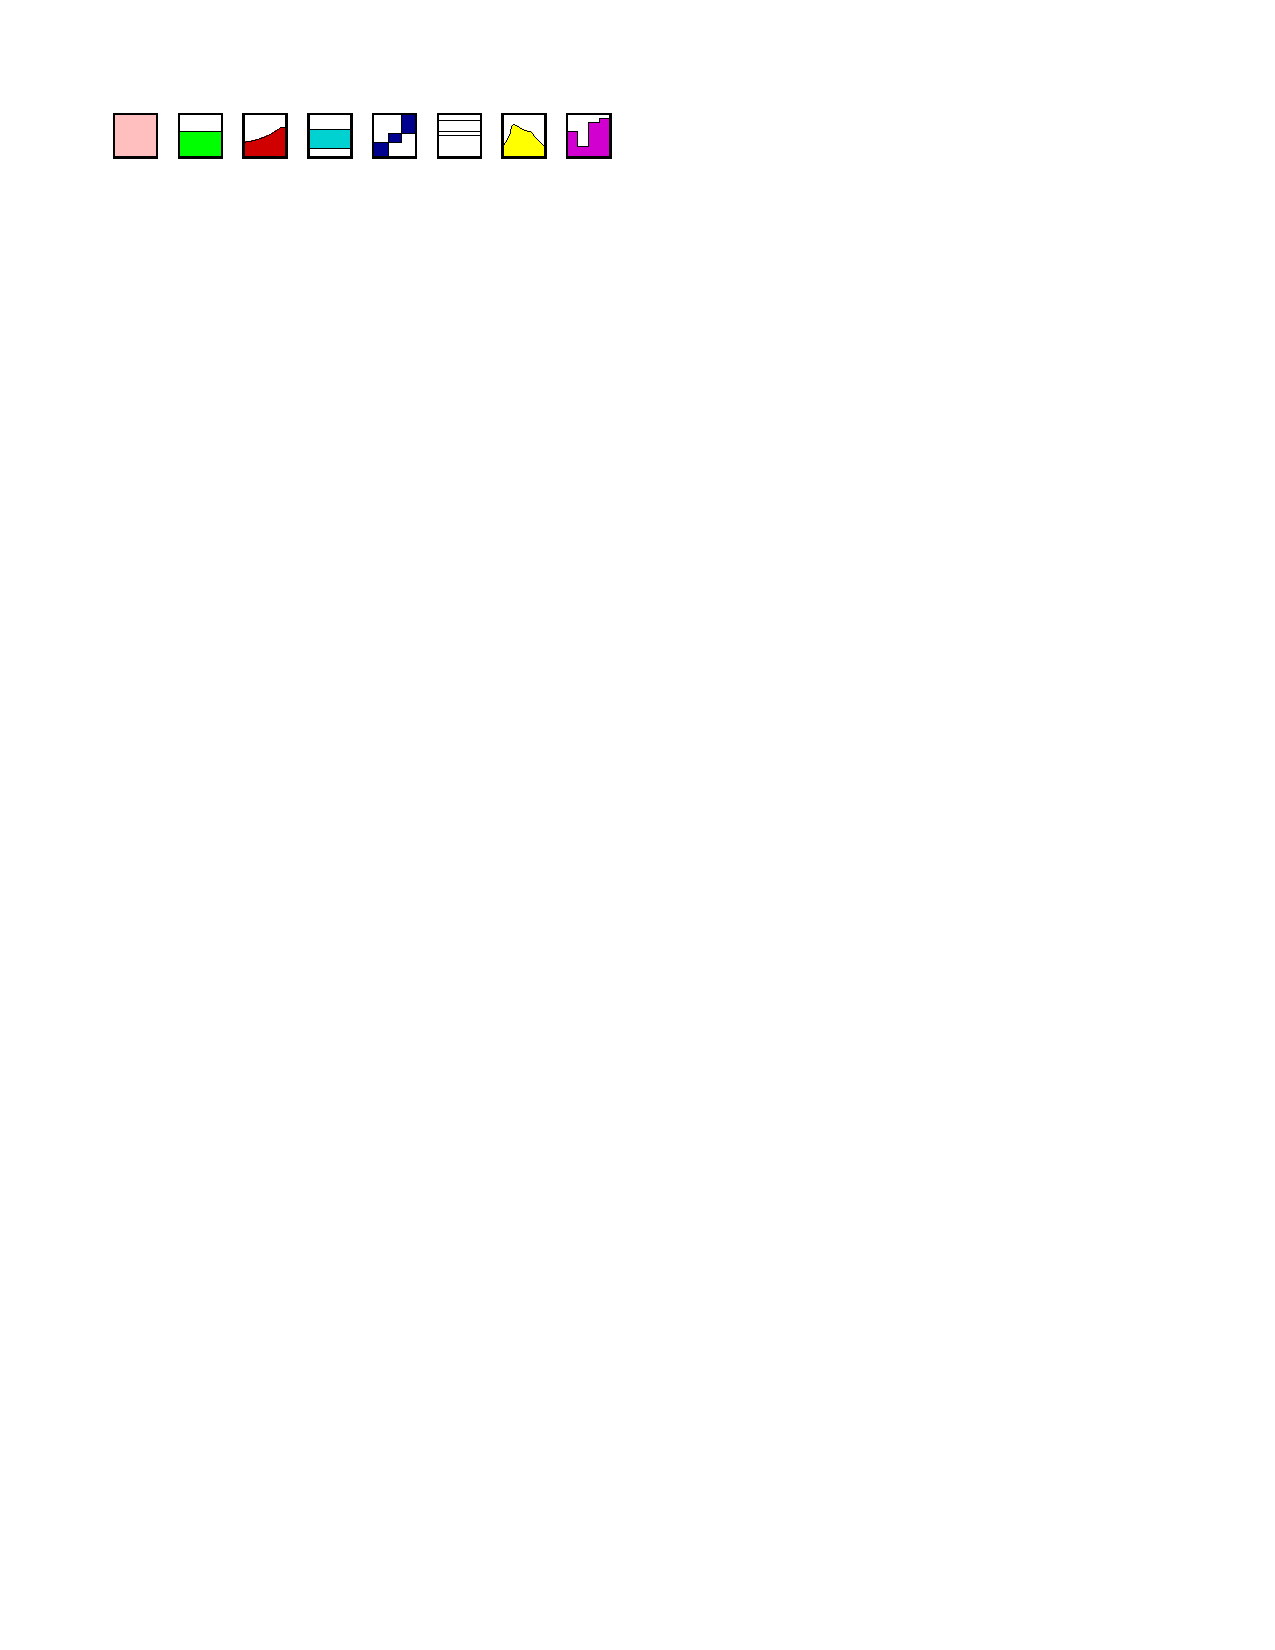
\includegraphics[width=0.65\textwidth]{figures/glyphs_zame.pdf}
    \caption{Eight different glyphs for aggregated edges (color shade,
average, min/max histogram, min/max range, min/max tribox, Tukey
box, smooth histogram, step histogram)~\cite{ElmqvistDGHF08}.}
    \label{fig:glyphs-zame}
  \end{center}
\end{figure}


\item \textbf{Pixel-oriented}

Pixel-oriented techniques display the most possible information at a time but mapping each attribute value of data to a single colored pixel. Color mapping approaches such as linear variation of brightness, maximum variation of hue and constant maximum saturation are used to color pixels which are arranged adequately in limited space. By providing an overview of large amounts of data, pixel-oriented display techniques are suitable for a variety of data mining tasks of large databases~\cite{zhang07thesis}.

The first pixel-oriented technique was presented by Keim~\cite{keim94pixel} as part of the VisDB system. Large amounts of multidimensional data could be represented as Spirals and Axes. Figure \ref{fig:pixel-spiral} illustrates how a spiral would be constructed and figure \ref{fig:pixel-axes} shows a rendered result of the axes technique. Further developments include the Recursive Pattern Technique \cite{keim95recpat} and the Circle Segments Technique \cite{Ankerst96circlesegments}. Figure \ref{fig:pixel-circle} visualizes such a circle which represents about 265,000 50-dimensional data items.

While no real-world examples have been identified during the research, using pixel-oriented techniques for visualizing complex clusters on a map seems possible. As the visualization relies on a large amounts of multidimensional data being present within clusters, the clustering algorithm would need to provide such required data. Performance implications also need to be considered, as potentially multiple clusters have to be visualized on a map, sometimes even in real-time.

\hspace*{-1cm}\parbox [h]{0.33\textwidth }{
    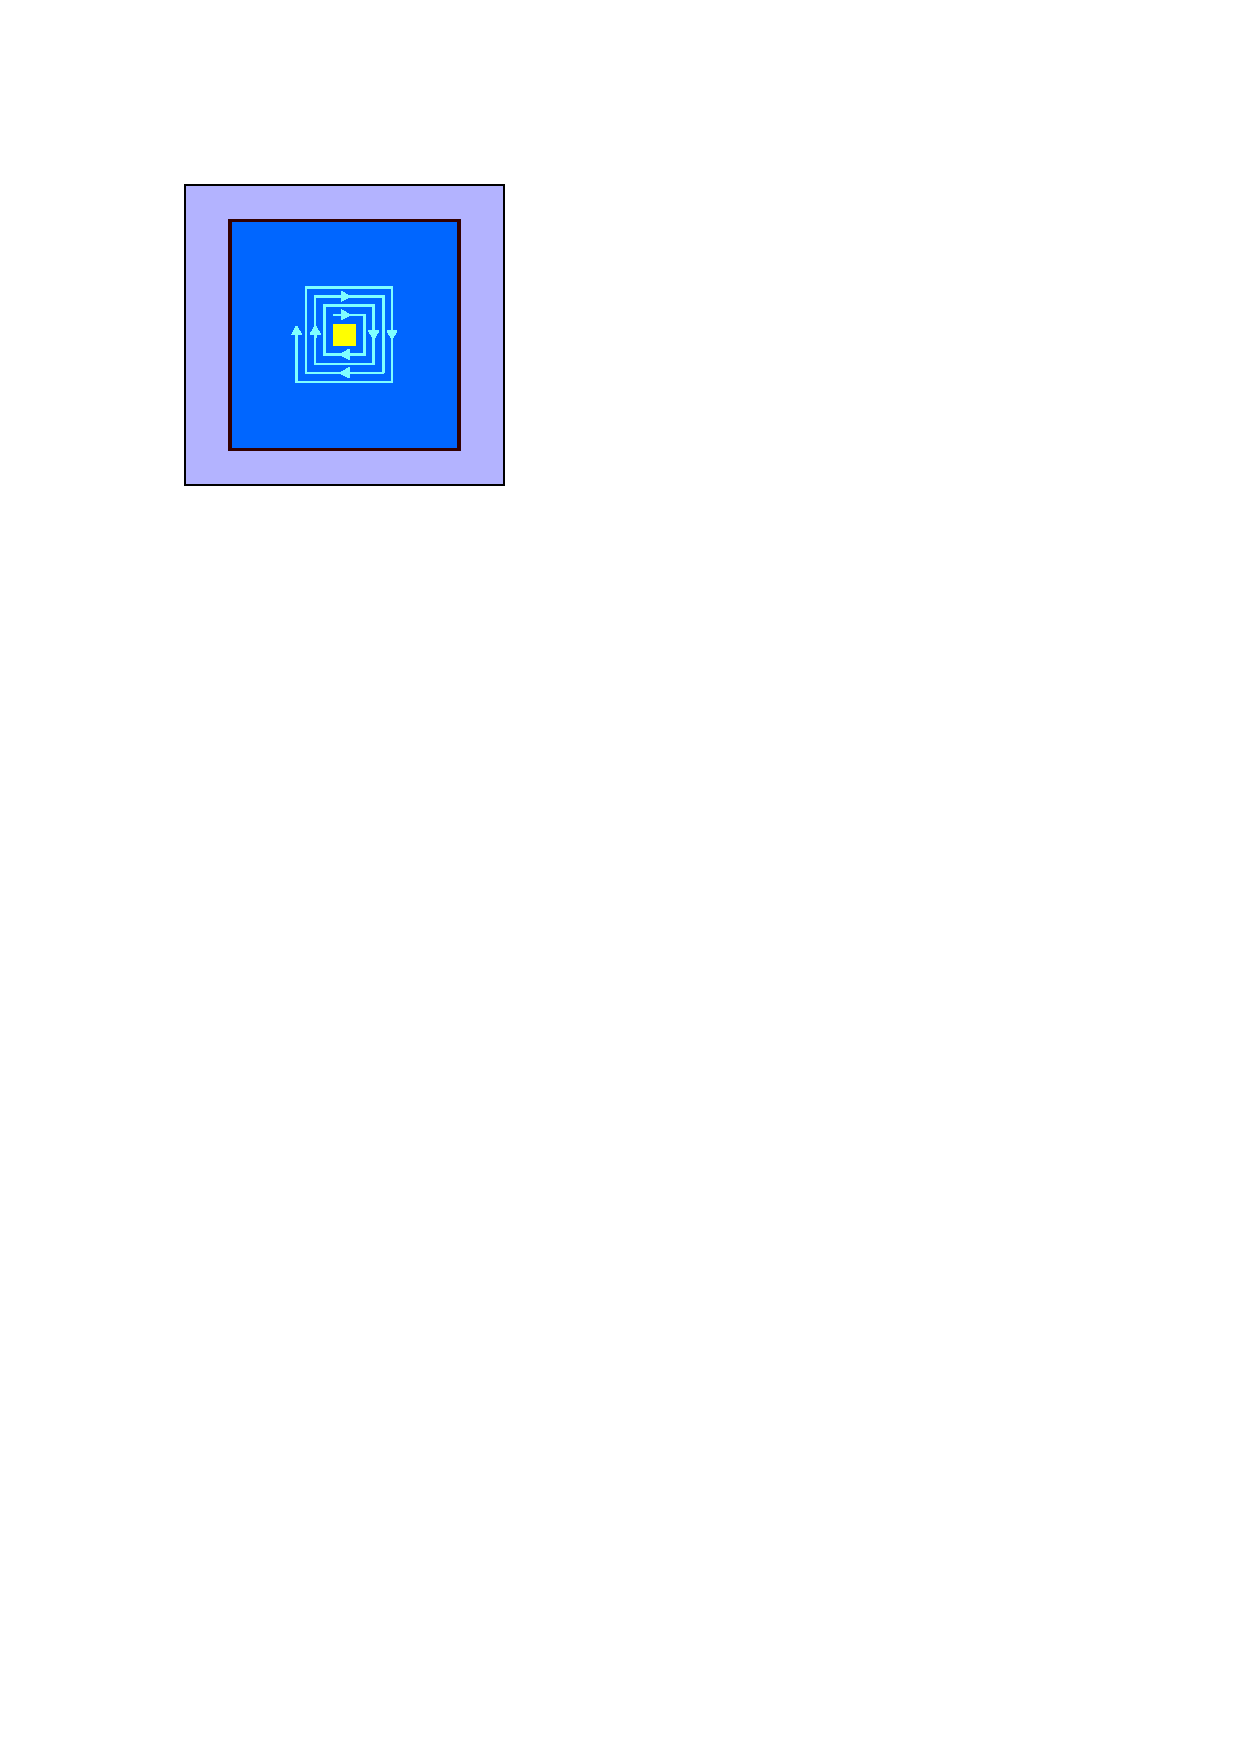
\includegraphics [width=\linewidth]{figures/pixel_keim_spiral.pdf}
    \captionof {figure}{Spiral~\cite{keim94pixel}}
    \label{fig:pixel-spiral}
}
\hfill
\hspace{0.2cm}
\parbox [h]{0.3\textwidth }{
    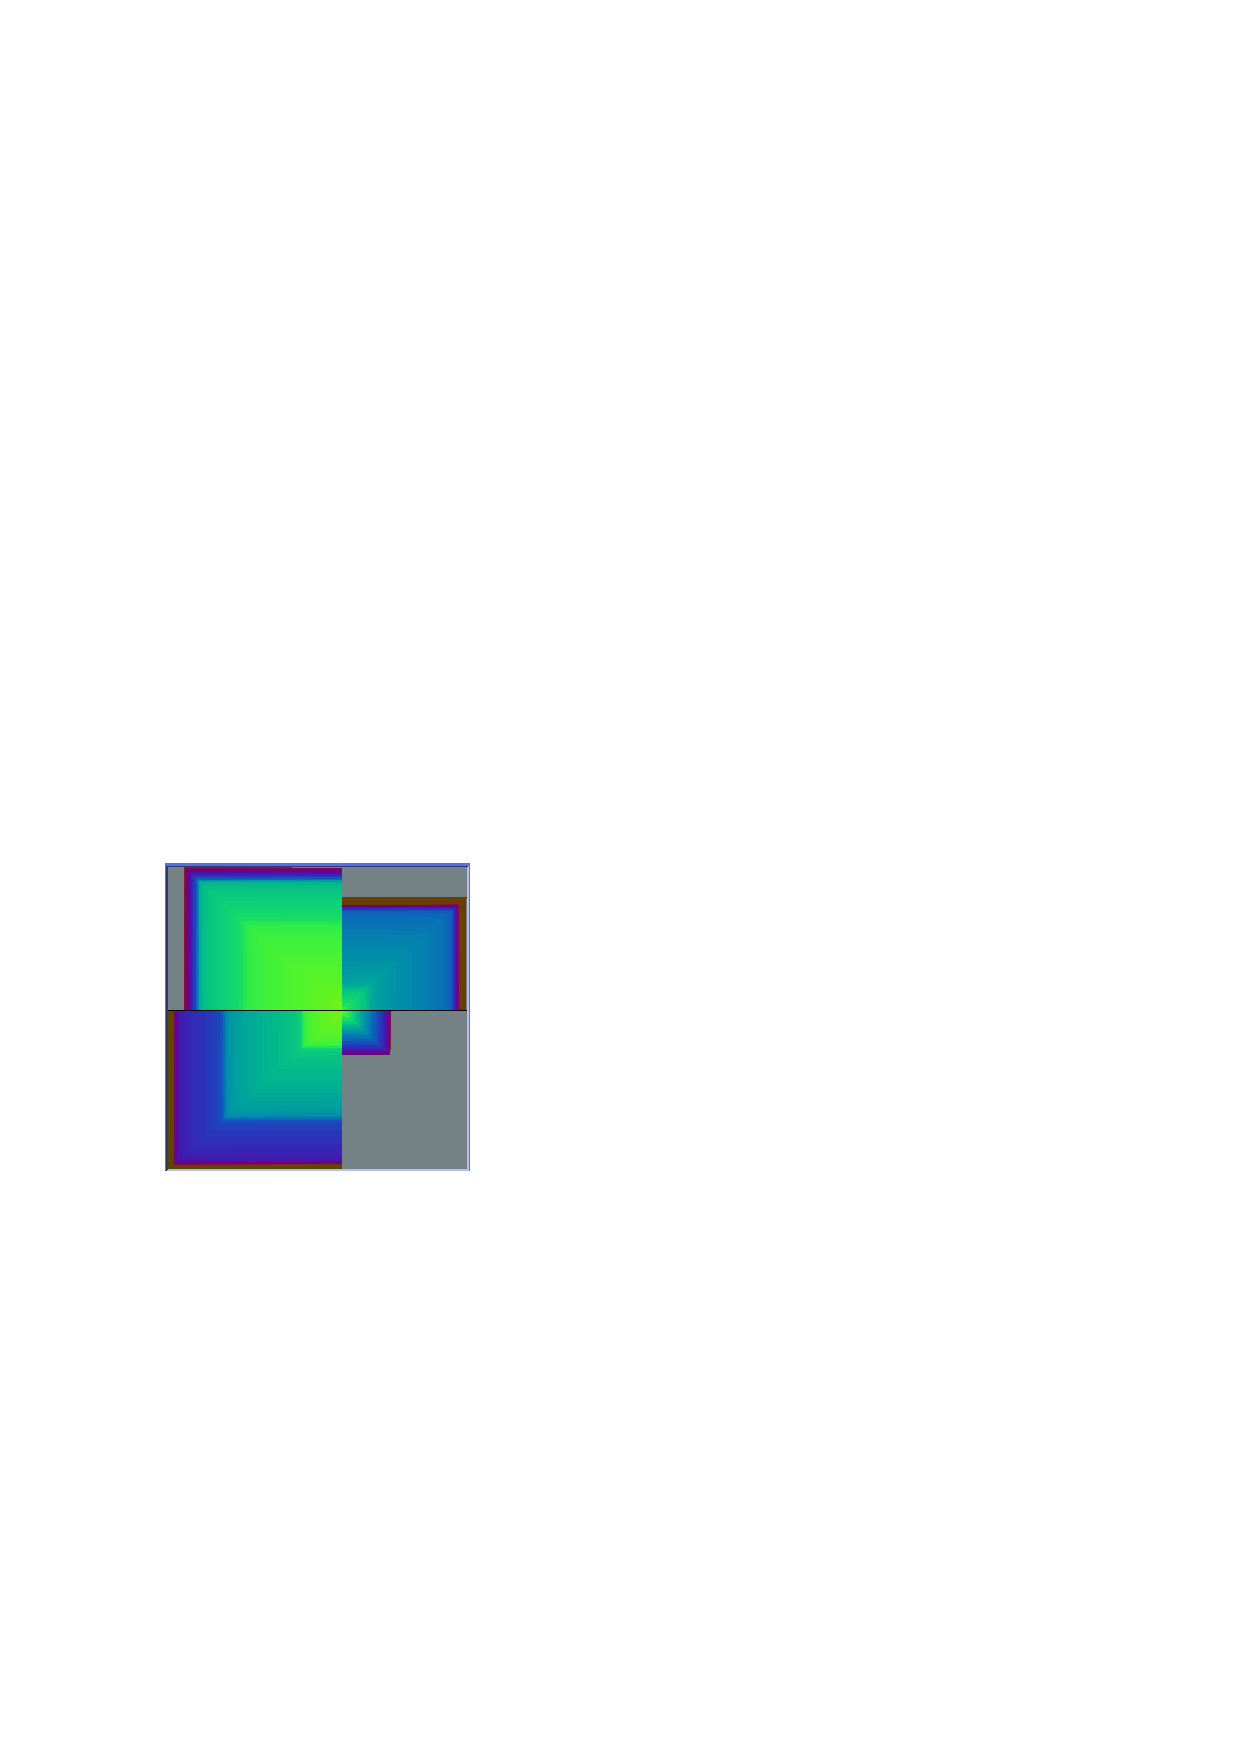
\includegraphics [width=\linewidth]{figures/pixel_keim_axes.pdf}
    \captionof {figure}{Axes \cite{keim94pixel}}
    \label{fig:pixel-axes}
}
\hfill
\hspace{0.2cm}
\parbox [h]{0.3\textwidth }{
    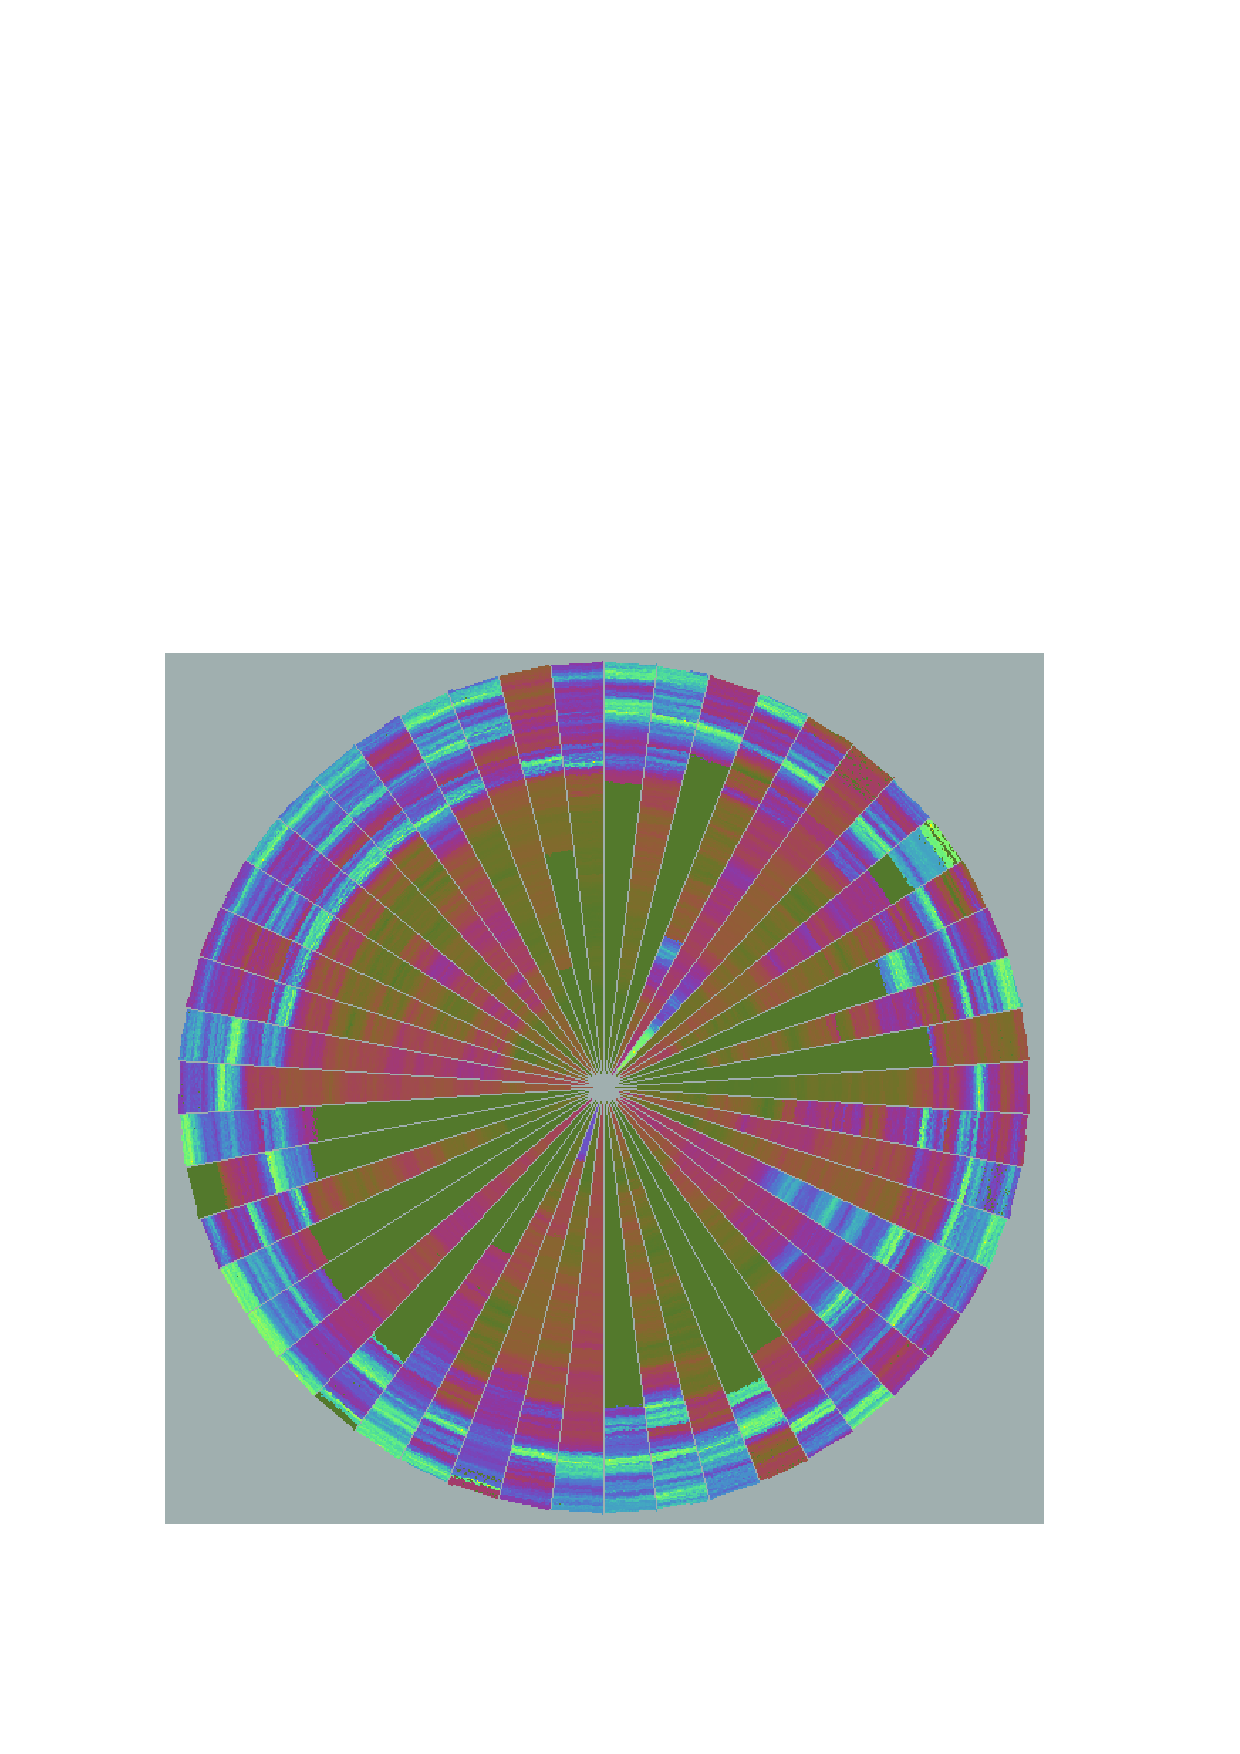
\includegraphics [width=\linewidth]{figures/pixel_keim_circle.pdf}
    \captionof {figure}{Circle \cite{Ankerst96circlesegments}}
    \label{fig:pixel-circle}
}


\item \textbf{Geometric techniques \& Diagrams}

Geometric techniques produce useful and insightful visualization by using geometric transformations and projects of the data.  Diagrams are algorithmically drawn graphics that visualize data. This section lists a selection of geometric techniques for multivariate data presented by Ke-Bing Zhang~\cite{zhang07thesis}, diagram types described by Dieter Ladenhauf~\cite{ladenhauf12dia} and related examples found in additional literature and on the web as stated in the individual references.

Line charts visualize data as lines by connecting data points of the corresponding values. They are used to display trends over time. Figure \ref{fig:did-map-sparklines} illustrates surface temperature anomalies from NASA's GISS as Spark line map~\cite{web:sparkmaps}. The Sparkline is a reduced line chart without axes and coordinates. It presents the general shape of variation in a simple and highly condensed way~\cite{wiki:sparkline}.


bar chart
http://www.ugandawatch.org/

pie chart
http://kartograph.org/showcase/charts/

map hull
\cite{Cristani08geoimagemaps}


\parbox [h]{0.4\textwidth }{
    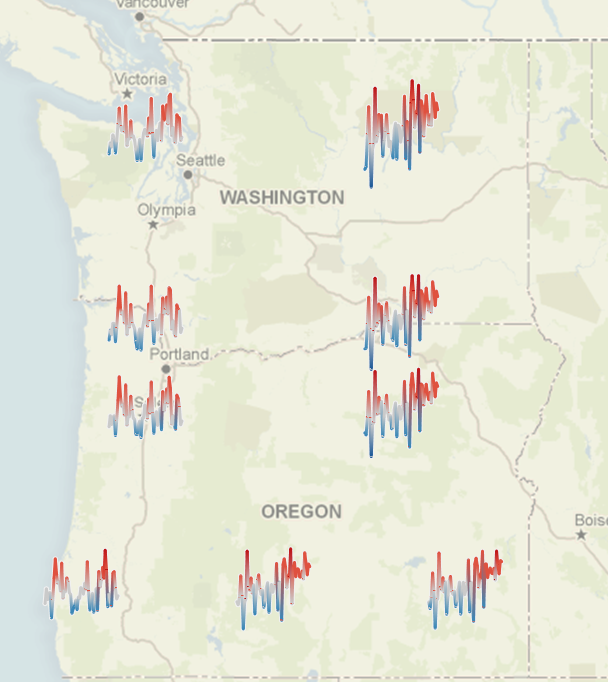
\includegraphics [width=\linewidth]{figures/dia_map_sparklines.png}
    \captionof {figure}{Spark line map}
    \label{fig:did-map-sparklines}
}
\hfill
\hspace{0.5cm}
\parbox [h]{0.4\textwidth }{
    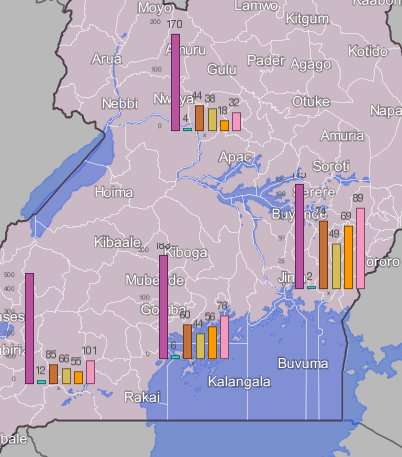
\includegraphics [width=\linewidth]{figures/dia_map_barchart.png}
    \captionof {figure}{Bar chart map}
    \label{fig:did-map-barchart}
}


\parbox [h]{0.4\textwidth }{
    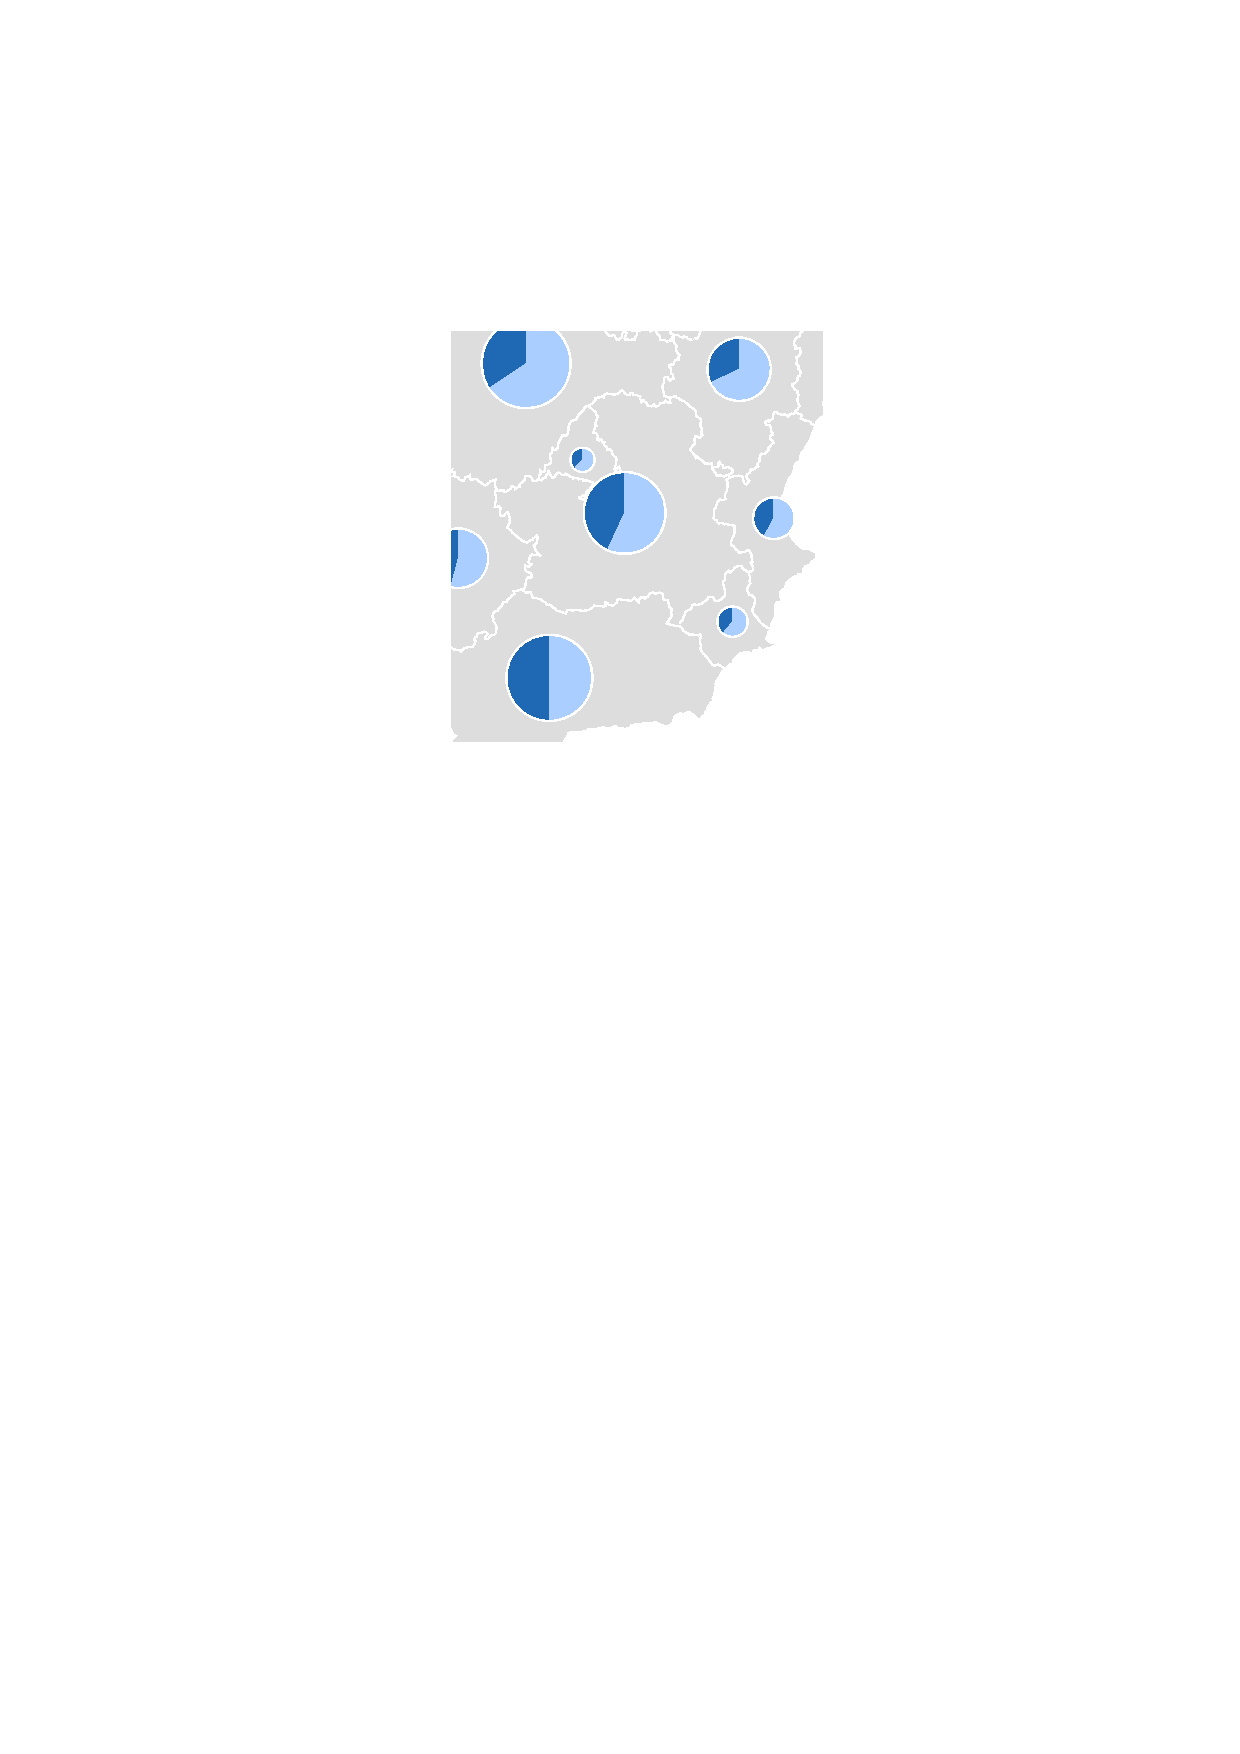
\includegraphics [width=\linewidth]{figures/dia_map_piechart.pdf}
    \captionof {figure}{Pie chart map}
    \label{fig:did-map-piechart}
}
\hfill
\hspace{0.5cm}
\parbox [h]{0.4\textwidth }{
    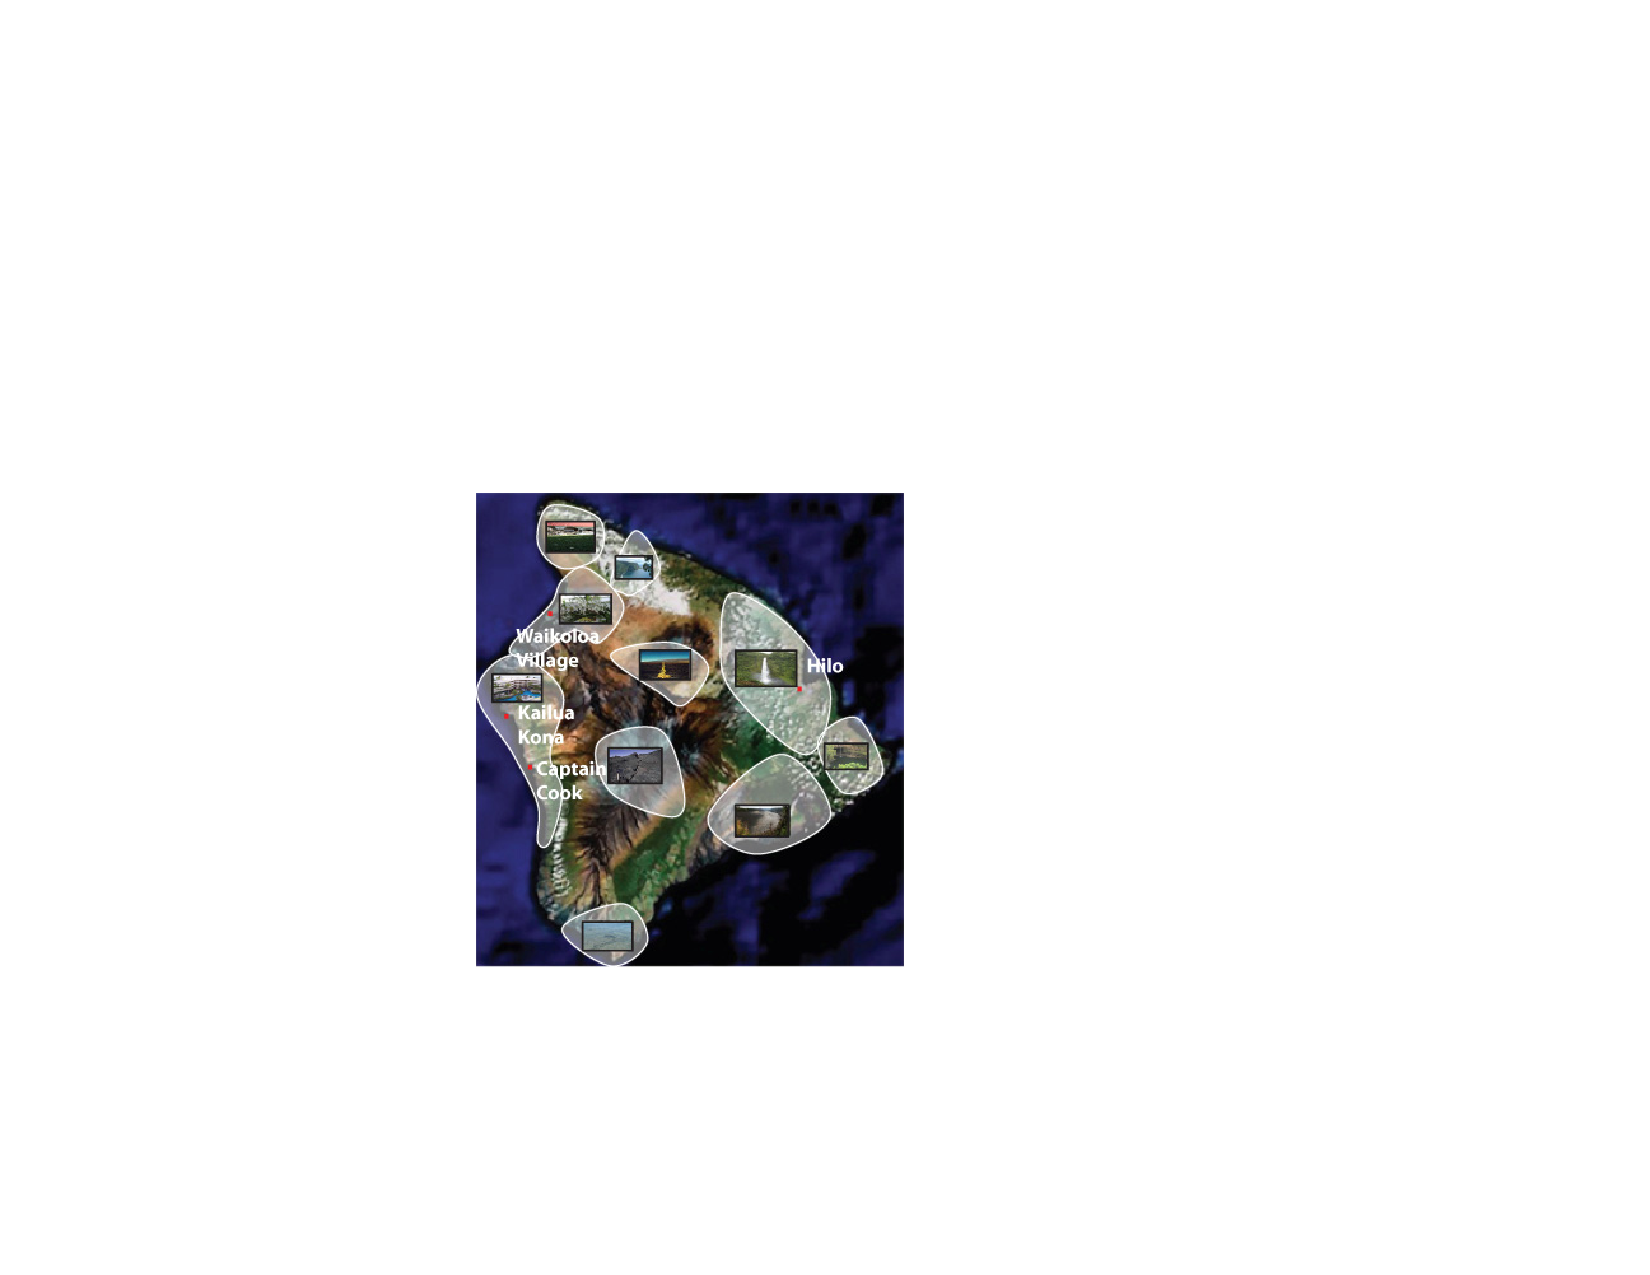
\includegraphics [width=\linewidth]{figures/dia_map_hull.pdf}
    \captionof {figure}{Convex hull map}
    \label{fig:did-map-hull}
}


\end{itemize}










